\chapter{Tiesioginis išvedimas}

\section{Užduotis}

Parašyti programą, kuri, kaip pradinius duomenis gavusi trejetą
$<R, F, G>$, panaudodama tiesioginio išvedimo sistemą nustatytų
ar tikslas $G$ yra išvedamas ir jei taip, tai kokias produkcijas
turime pritaikyti, kad jį gautume.

\section{Pseudo kodas}

\label{sec:fc:pseudo}

Pradiniai duomenys:
\begin{description}
  \item[$R$] – taisyklių sąrašas;
  \item[$F$] – pradinių faktų aibė;
  \item[$G$] – ieškomas tikslas.
\end{description}

Rezultatas:
\begin{description}
  \item[$Q$] – panaudotų taisyklių seka.
\end{description}

\begin{algorithmic}[1]
  \Function{tiesioginis išvedimas}{$R, F, G$}
    \State $Q := \left(  \right)$
    \State $r :=$ pirma iš taisyklių;
    \While{yra pritaikomų taisyklių $\land G \not\in F$}
                                        \label{fc:pseudo:while_condition}
      \If{$r$ prielaidos yra tarp $F \land r$ išvados nėra tarp $F$}
                                        \label{fc:pseudo:if_condition}
        \State $r$ išvadą pridedame į $F$;
                                        \label{fc:pseudo:add_fact}
        \State $r := $ pirma iš taisyklių;
                                        \label{fc:pseudo:start}
        \State $r$ pridedame į $Q$ galą;
                                        \label{fc:pseudo:add_rule}
      \Else
        \State $r := $ kita taisyklė;   \label{fc:pseudo:next_rule}
      \EndIf
    \EndWhile
    \State \Return Q;
  \EndFunction
\end{algorithmic}

\section{Realizacija}

Tiesioginio išvedimo algoritmo, pateikto \ref{sec:fc:pseudo}
skyrelyje, realizacija:

\pythonai{source}{forwardchaining.ForwardChaining.run}

\section{Pavyzdžiai}

\subsection{Pirmasis pavyzdys: paprastas atvejis}

\begin{pythonaienv}[fc]
# Vytauto Astrausko failas.
1. Taisyklės.
ZFB                                     # R1: F, B → Z
FCD                                     # R2: C, D → F
DA                                      # R3: A → D

2. Faktai.
ACB

3. Tikslas.
Z
\end{pythonaienv}

\subsection{Antrasis pavyzdys: du išvedimo keliai}

\begin{pythonaienv}[fc]
# Taisyklės:
D Z                                     # R1: D → Z
C D                                     # R2: C → D
B C                                     # R3: B → C
A G                                     # R4: A → G
G Z                                     # R5: G → Z
A B                                     # R6: A → B
# Faktai:
A
# Tikslas:
Z
\end{pythonaienv}

\subsection{Trečiasis pavyzdys: du išvedimo keliai (taisyklės kita tvarka)}

\begin{pythonaienv}[fc]
# Taisyklės:
A G                                     # R1: A → G
D Z                                     # R2: D → Z
C D                                     # R3: C → D
B C                                     # R4: B → C
A B                                     # R5: A → B
G Z                                     # R6: G → Z
# Faktai:
A
# Tikslas:
Z
\end{pythonaienv}

\subsection{Ketvirtasis pavyzdys: didesnis testas}

\begin{pythonaienv}[fc]
# Taisyklės:
FB Z                                    # R1: F, B → Z
CD F                                    # R2: C, D → F
A D                                     # R3: A → D
A L                                     # R4: A → L
L K                                     # R5: L → K
B A                                     # R6: B → A
D M                                     # R7: D → M
# Faktai:
ABC
# Tikslas:
Z
\end{pythonaienv}

\subsection{Penktasis pavyzdys: ilgas antecedentas}

\begin{pythonaienv}[fc]
# Taisyklės:
G Z                                     # R1: G → Z
A G                                     # R2: A → G
A B                                     # R3: A → B
B C                                     # R4: B → C
C D                                     # R5: C → D
D Z                                     # R6: D → Z
ABGCDZ H                                # R7: A, B, C, D, G, Z → H
# Faktai:
A
# Tikslas:
H
\end{pythonaienv}

\subsection{Šeštasis pavyzdys: išvedimas neegzistuoja}

\begin{pythonaienv}[fc]
# Taisyklės:
CD F                                    # R1: C, D → F
A D                                     # R2: A → D
A L                                     # R3: A → L
L K                                     # R4: L → K
B A                                     # R5: B → A
D M                                     # R6: D → M
FB Z                                    # R7: F, B → Z
# Faktai:
ABC
# Tikslas:
H
\end{pythonaienv}

\subsection{Septintasis pavyzdys: tikslas tarp prielaidų}

\begin{pythonaienv}[fc]
# Taisyklės:
CD F                                    # R1: C, D → F
A D                                     # R2: A → D
A L                                     # R3: A → L
L K                                     # R4: L → K
B A                                     # R5: B → A
D M                                     # R6: D → M
FB Z                                    # R7: F, B → Z
# Faktai:
ABC
# Tikslas:
B
\end{pythonaienv}

\subsection{Aštuntasis pavyzdys: devynių produkcijų DC}

\begin{pythonaienv}[fc]
# Vytauto Astrausko failas.
1. Taisyklės.
ZDC                                     # R1: D, C → Z
DC                                      # R2: C → D
CB                                      # R3: B → C
BA                                      # R4: A → B
AD                                      # R5: D → A
DT                                      # R6: T → D
AG                                      # R7: G → A
BH                                      # R8: H → B
CJ                                      # R9: J → C

2. Faktai.
T

3. Tikslas.
Z
\end{pythonaienv}

\subsection{Devintasis pavyzdys: devynių produkcijų CD}

\begin{pythonaienv}[fc]
# Vytauto Astrausko failas.
1. Taisyklės.
ZCD                                     # R1: C, D → Z
DC                                      # R2: C → D
CB                                      # R3: B → C
BA                                      # R4: A → B
AD                                      # R5: D → A
DT                                      # R6: T → D
AG                                      # R7: G → A
BH                                      # R8: H → B
CJ                                      # R9: J → C

2. Faktai.
T

3. Tikslas.
Z
\end{pythonaienv}

\subsection{Dešimtasis pavyzdys: labirintas}

\subsubsection{Labirinto žemėlapis}

\begin{figure}[H]
  \centering
  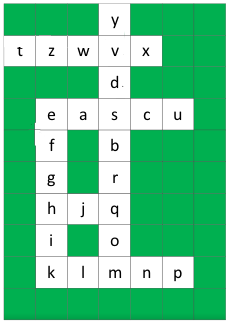
\includegraphics[]{content/map.png}
  \caption{Labirinto žemėlapis}
  \label{fig:fc:map}
\end{figure}

\begin{pythonaienv}[fc]
# Vytauto Astrausko failas.
1. Taisyklės.
Ft                                      # R1: t → F
Fy                                      # R2: y → F
ds                                      # R3: s → d
sd                                      # R4: d → s
as                                      # R5: s → a
sa                                      # R6: a → s
bs                                      # R7: s → b
sb                                      # R8: b → s
cs                                      # R9: s → c
sc                                      # R10: c → s
vd                                      # R11: d → v
dv                                      # R12: v → d
yv                                      # R13: v → y
vy                                      # R14: y → v
wv                                      # R15: v → w
vw                                      # R16: w → v
xv                                      # R17: v → x
vx                                      # R18: x → v
wz                                      # R19: z → w
zw                                      # R20: w → z
tz                                      # R21: z → t
zt                                      # R22: t → z
ea                                      # R23: a → e
ae                                      # R24: e → a
fe                                      # R25: e → f
ef                                      # R26: f → e
gf                                      # R27: f → g
fg                                      # R28: g → f
hg                                      # R29: g → h
gh                                      # R30: h → g
ih                                      # R31: h → i
hi                                      # R32: i → h
jh                                      # R33: h → j
hj                                      # R34: j → h
ki                                      # R35: i → k
ik                                      # R36: k → i
lk                                      # R37: k → l
kl                                      # R38: l → k
ml                                      # R39: l → m
lm                                      # R40: m → l
om                                      # R41: m → o
mo                                      # R42: o → m
nm                                      # R43: m → n
mn                                      # R44: n → m
qo                                      # R45: o → q
oq                                      # R46: q → o
rq                                      # R47: q → r
qr                                      # R48: r → q
jq                                      # R49: q → j
qj                                      # R50: j → q
br                                      # R51: r → b
rb                                      # R52: b → r
pn                                      # R53: n → p
np                                      # R54: p → n
uc                                      # R55: c → u
cu                                      # R56: u → c

2. Faktai.
s

3. Tikslas.
F
\end{pythonaienv}
